%  http://latex-beamer.sourceforge.net/

%\documentclass[landscape]{foils}

%\documentclass{beamer}
%\documentclass[handout]{beamer}     % TO PRINT PRESENTATION HANDOUT
\documentclass[xcolor=dvipsnames]{beamer}  % ALLOWS CHANGE IN COLOR

\usepackage{pifont} %para tener la ballot cross \ding{55}

\usepackage{beamerthemesplit}
\usepackage{url}
\usepackage{ae} % or {zefonts}
\usepackage[T1]{fontenc}
\usepackage[ansinew]{inputenc}
\usepackage[spanish,es-nodecimaldot]{babel}

\usepackage{amsmath}

\usepackage{graphicx}
\graphicspath{"../graphs/"}
\usepackage{color}
%\usepackage[colorlinks]{hyperref} % beamer loads this by default, needed only to change default behavior? 
\usepackage{tikz} % Easier syntax to draw pgf files (invokes pgf automatically)
\usetikzlibrary{arrows,shapes.geometric}

\usepackage{tabulary} % automatic column length in tables with long text string
%% use LRJC for auto, and lrjc for normal column width
\setlength\tymin{10pt}       %% change behavior, see p. 254 LaTeX companion
\setlength\tymax{\maxdimen}  %% change behavior, see p. 254 LaTeX companion

\usepackage{multirow} %allows multiple rows in tables

%\usecolortheme{crane}     %Color yellow
%\usetheme{Warsaw}
\usecolortheme[named=Gray]{structure}

\useoutertheme[footline=empty]{}  % PUTS COLORED LINE AT FOOT WITH TITLE, AUTHOR, PAGE, etc
%\usetheme{Berkeley}
\usetheme[height=7mm]{Rochester}
\setbeamertemplate{items}[ball]   % ITEMS IN 3D BALLS (alt CIRCLES)
\setbeamertemplate{navigation symbols}{}  % DROPS NAVIGATION ICONS
\setbeamertemplate{blocks}[rounded][shadow=true]

%\setbeamertemplate{footline} {
%    \begin{beamercolorbox}{section in head/foot}
%    \insertsectionnavigationhorizontal{\paperwidth}{}{plus1filll
%    \insertframenumber}
%    \end{beamercolorbox}
%}

%\setbeamertemplate{navigation symbols}{\insertslidenavigationsymbol,
%\insertdocnavigationsymbol} \setbeamertemplate{footline} {
%    \begin{beamercolorbox}{section in head/foot}
%    \insertsectionnavigationhorizontal{\paperwidth}{}{plus1filll
%    \insertframenumber}
%    \end{beamercolorbox}
%}

\setbeamercovered{transparent}
\setbeamertemplate{caption}{\insertcaption}
\setbeamertemplate{footline}[frame number] % adds slide number, overrides split footer with authors/title that the theme uses

\tikzstyle{nodo} = [circle, draw=black, fill=white, text=black]
\tikzstyle{end} = [circle, minimum width=3pt,fill, inner sep=0pt]

\title[Malapportionment \& bias]{Malapportionment and representation}
\subtitle{Party bias and responsiveness in Mexico}
\author[Magar, Altman, McDonald, Trelles]{E. Magar\inst{1} \and M. Altman\inst{2} \and M.P. McDonald\inst{3} \and A. Trelles\inst{4}}
\institute[ITAM-MIT-UFG-Pitt]{\inst{1} ITAM \and 
                              \inst{2} MIT \and
                              \inst{3} UF, Gainesville \and
                              \inst{4} University of Pittsburgh}
%\address{}
\date[14nov14]{Analyzing Latin American Politics Conference\\ University of Houston \\ 11/14/14}

\begin{document}

%%%%%%%%%%%%%%%%%%%%%%%%%%%%%%%%%%%%%%%%%%%%%%%%%%%%%%%%%%%%%%%%%%%%%%%%%%%%%%%%%%%%%%%%%%%%

\frame[plain]{\titlepage}

%%%%%%%%%%%%%%%%%%%%%%%%%%%%%%%%%%%%%%%%%%%%%%%%%%%%%%%%%%%%%%%%%%%%%%%%%%%%%%%%%%%%%%%%%%%%
\begin{frame}                      % SLIDE

    \frametitle{How does malapportionment distort representation?}


Sparsely populated areas get same representation as the densely populated
%\emph{\textbf{Q:}} What can we learn from the Mexico City legislative assembly?
%How does malapportionment distort representation? \\
%(Erikson 1972, Tufte 1973)


\bigskip

Studies of U.S.\ and U.K.\  

\begin{itemize}

\item instills bias when one party strong in small districts \\ (as Tories were up to 1997, Johnston 2002)

\item Reapportionment Revolution removed bias in \\ different, predictable degrees (Cox\&Katz 2002)

\item no party bias from malapp.\ after mid-1960s \\ (Grofman et al.~1997)

\end{itemize}

\bigskip

\pause

\begin{block}{How does Mexico fare?}

\begin{enumerate}
\item malapportionment? Substantial

\item Party bias? Not much, but big large-party bonus

\end{enumerate}

\end{block}

\end{frame}
%%%%%%%%%%%%%%%%%%%%%%%%%%%%%%%%%%%%%%%%%%%%%%%%%%%%%%%%%%%%%%%%%%%%%%%%%%%%%%%%%%%%%%%%%%%% 

\begin{frame}                      % SLIDE

    \frametitle{Mexican congressional districts}

Redistricting in 1997, 2006, and 2015 (abandoned)

\bigskip

Redistricting process (FPTP):
\begin{enumerate}
\item apportionment of 300 seats to 32 states
\item optimization algorithm $\rightarrow$ proposal
\item parties propose amendments (must improve score)
\item repeat 2 and 3
\item new map
\end{enumerate}

\bigskip

Redistricting by experts, but behind closed doors

\begin{multline*}
\texttt{Score} = .4 \times \texttt{PopBalance} + .3 \times \texttt{MunicBoundaries} \\
+ .2 \times \texttt{TravelTime} + .1 \times \texttt{Compactness}
\end{multline*}


Topic will be salient when single-term limits dropped in 2015

\end{frame}
%%%%%%%%%%%%%%%%%%%%%%%%%%%%%%%%%%%%%%%%%%%%%%%%%%%%%%%%%%%%%%%%%%%%%%%%%%%%%%%%%%%%%%%%%%%% 
\begin{frame}\label{fr:MxMapProj}                      % SLIDE

    \frametitle{The bigger project}

\emph{Draw Mexico} project = offspring of \emph{Public Mapping Project in U.S.}

\bigskip

Remove opaqueness from redistricting process 

\bigskip

\texttt{DistrictBuilder} is software (open-source)%({\footnotesize \url{www.districtbuilder.org}}):

\begin{itemize}

\item enables widespread DIY redistricting thru cloud computing

\item  internet lets anyone draw/inspect maps: crowdsourcing

\item redistricting contests in 6 states $\rightarrow$ hundreds of legal plans

\end{itemize}

\bigskip

Application to \alert{Mexico} \href{http://23.21.151.172/}{\beamergotobutton{Link: MexDemo}} \pause (Donations?) 

\end{frame}
%%%%%%%%%%%%%%%%%%%%%%%%%%%%%%%%%%%%%%%%%%%%%%%%%%%%%%%%%%%%%%%%%%%%%%%%%%%%%%%%%%%%%%%%%%%% 

\begin{frame}                      % SLIDE
    \frametitle{Apportionment}


Hamilton method used:

\begin{itemize}
\item The quota (or price of a seat) is $Q = \frac{\text{nation's population}}{300}$

\item First allocation is $\frac{\text{state's population}}{Q}$, rounded down

\item Every state gets 2 seats min. + indigenous voting rights

\item Unallocated seats, if any, awarded to states with largest fractional remainders
\end{itemize}

\bigskip

\pause

Most recent decennial census must be used 

\begin{itemize}
\item ... but no obligation to redistrict as soon as available
\item 6-year lag on average: 199\textbf{7}, 200\textbf{6}, 201\textbf{5}    
\item and IFE considers $\pm15\%$ imbalance normal (!)
\end{itemize}

\end{frame}

%%%%%%%%%%%%%%%%%%%%%%%%%%%%%%%%%%%%%%%%%%%%%%%%%%%%%%%%%%%%%%%%%%%%%%%%%%%%%%%%%%%%%%%%%%%% 

\begin{frame}                      % SLIDE
    \frametitle{Malapportionment between states}

\begin{center}
   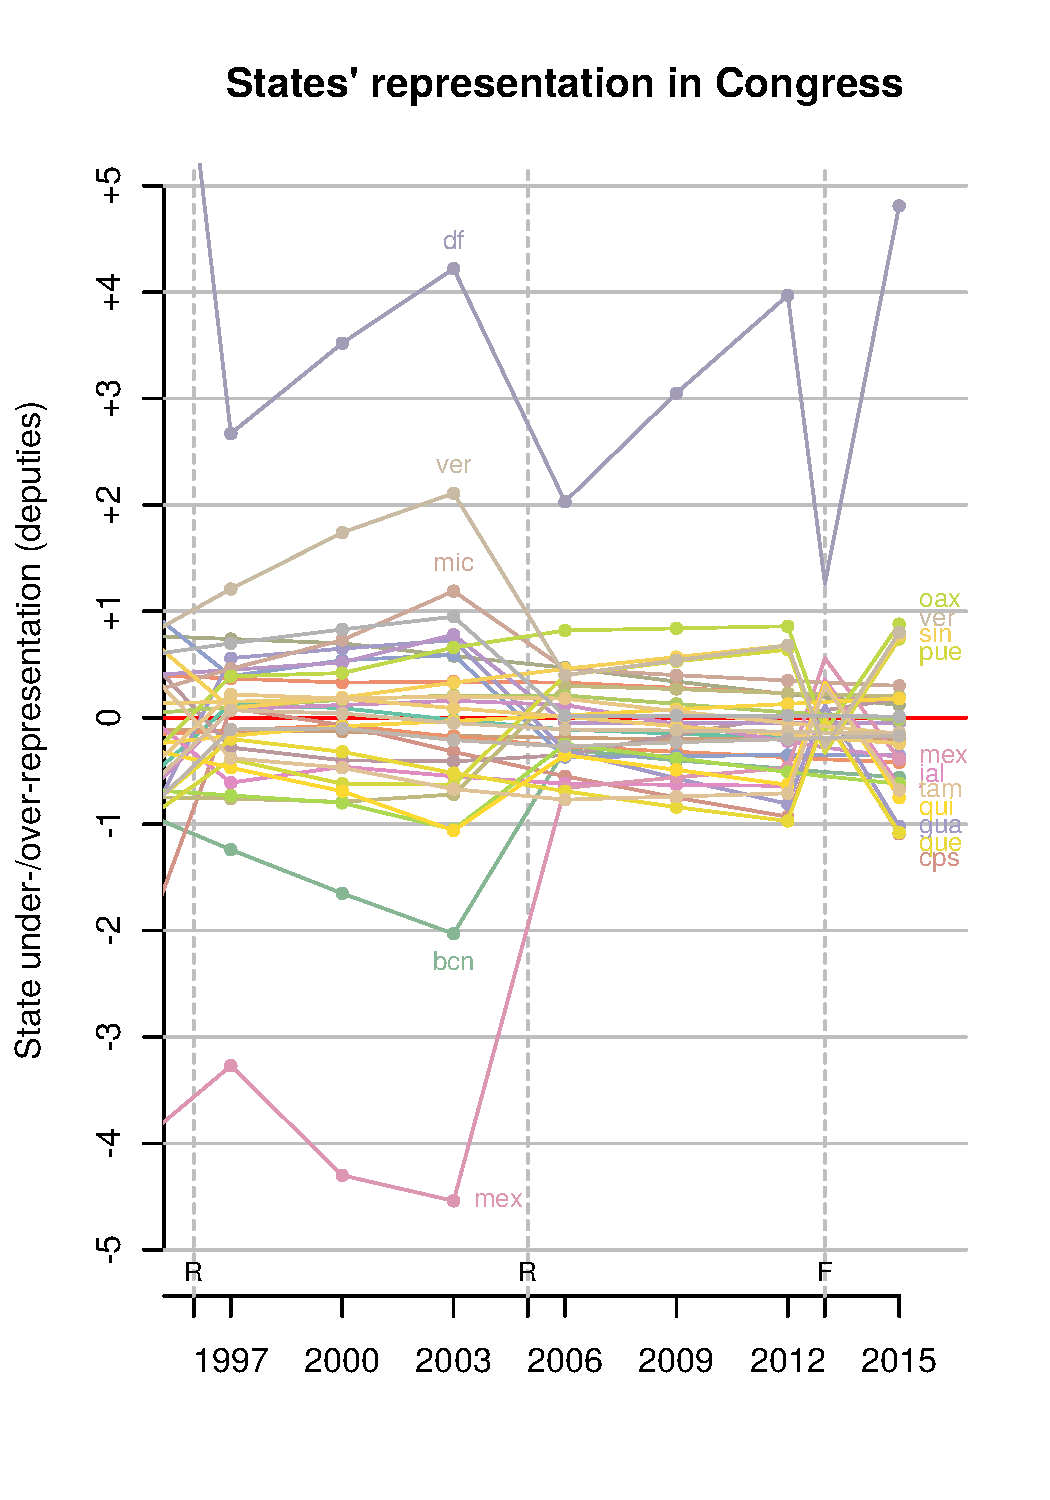
\includegraphics[width=6cm]{../graphs/statesUnderOverRep.pdf}
\end{center}

\end{frame}
%%%%%%%%%%%%%%%%%%%%%%%%%%%%%%%%%%%%%%%%%%%%%%%%%%%%%%%%%%%%%%%%%%%%%%%%%%%%%%%%%%%%%%%%%%%% 

\frame {                      % SLIDE
    \frametitle{Malapportionment between states}

\begin{center}
   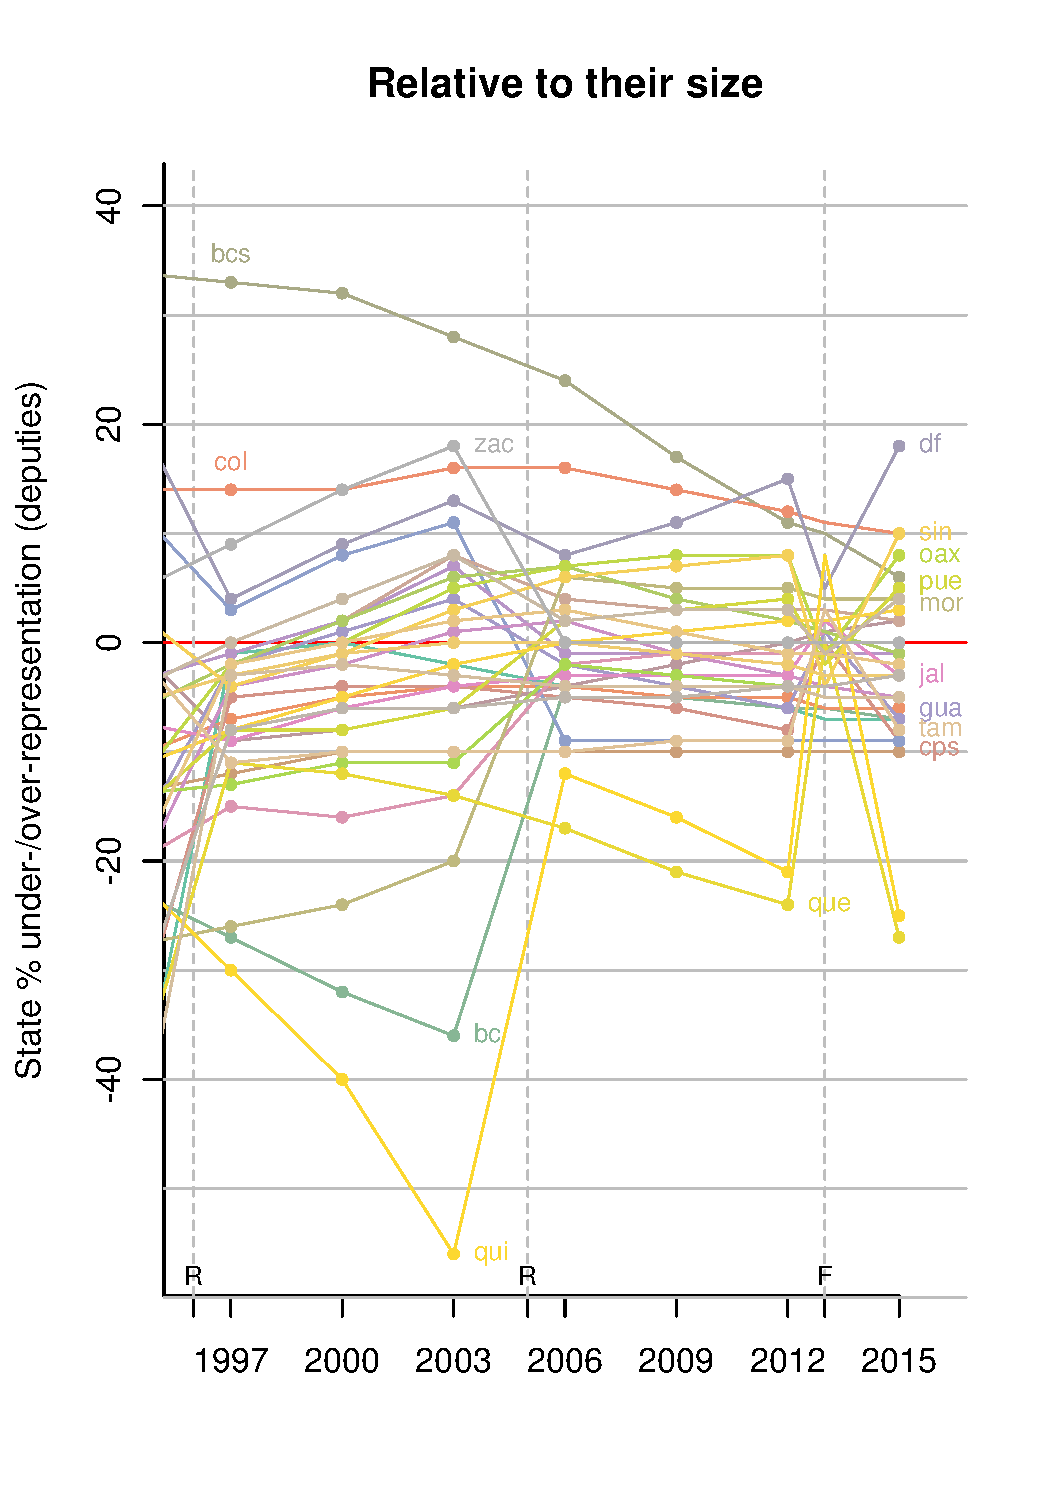
\includegraphics[width=6cm]{../graphs/statesUnderOverRep-rel.pdf}
\end{center}

}
%%%%%%%%%%%%%%%%%%%%%%%%%%%%%%%%%%%%%%%%%%%%%%%%%%%%%%%%%%%%%%%%%%%%%%%%%%%%%%%%%%%%%%%%%%%% 

\frame {                      % SLIDE
    \frametitle{Malapportionment within states}

\begin{center}
   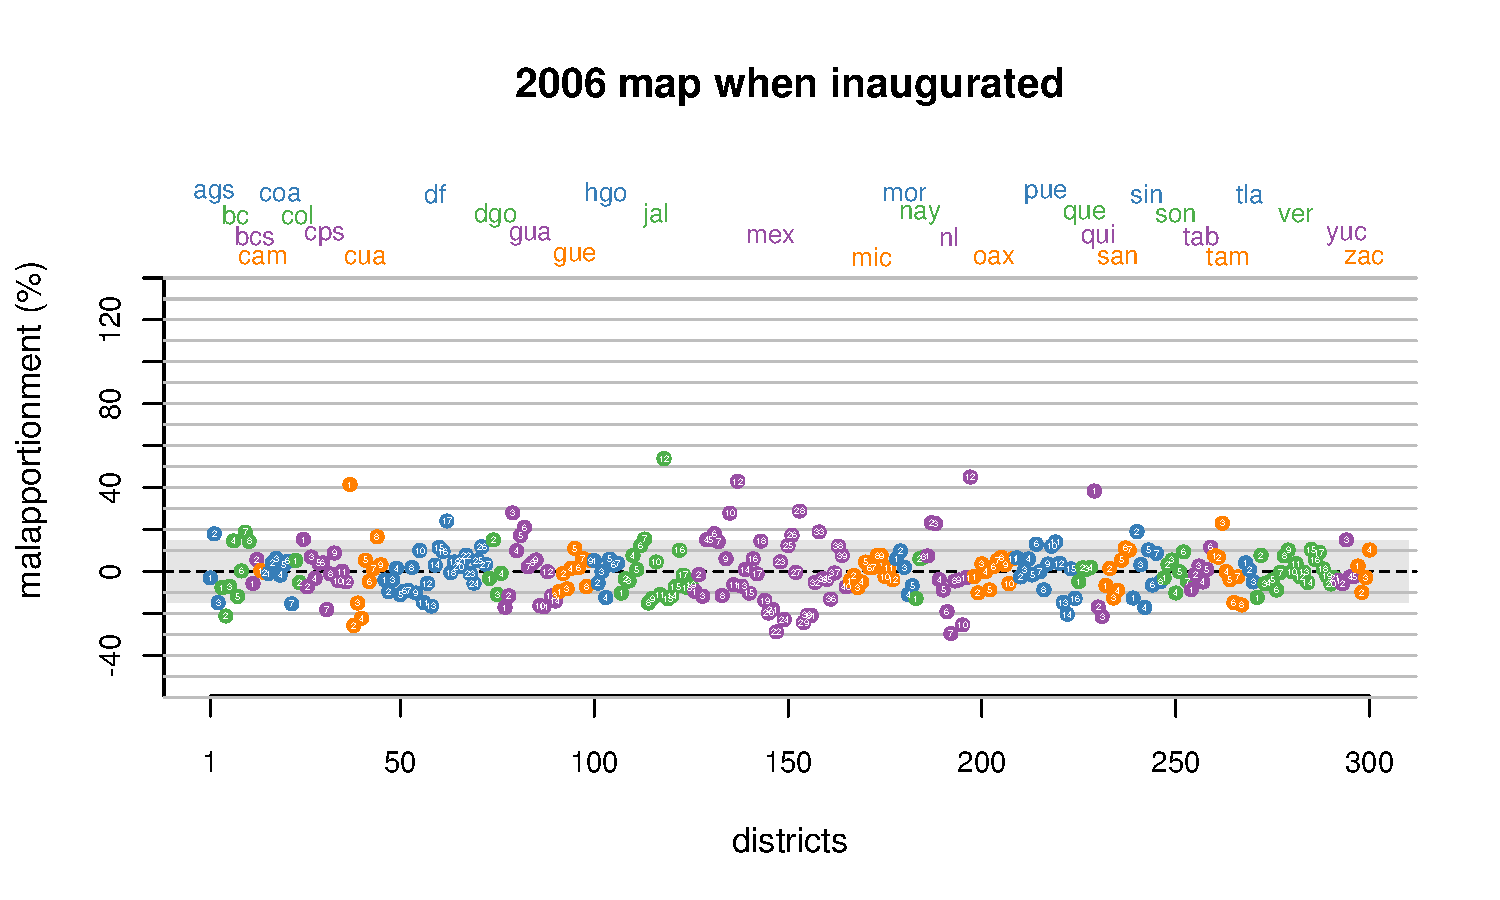
\includegraphics[width=12cm]{../graphs/malapp2006d0.pdf}
\end{center}

}
%%%%%%%%%%%%%%%%%%%%%%%%%%%%%%%%%%%%%%%%%%%%%%%%%%%%%%%%%%%%%%%%%%%%%%%%%%%%%%%%%%%%%%%%%%%% 

\frame {                      % SLIDE
    \frametitle{Malapportionment within states}

\begin{center}
   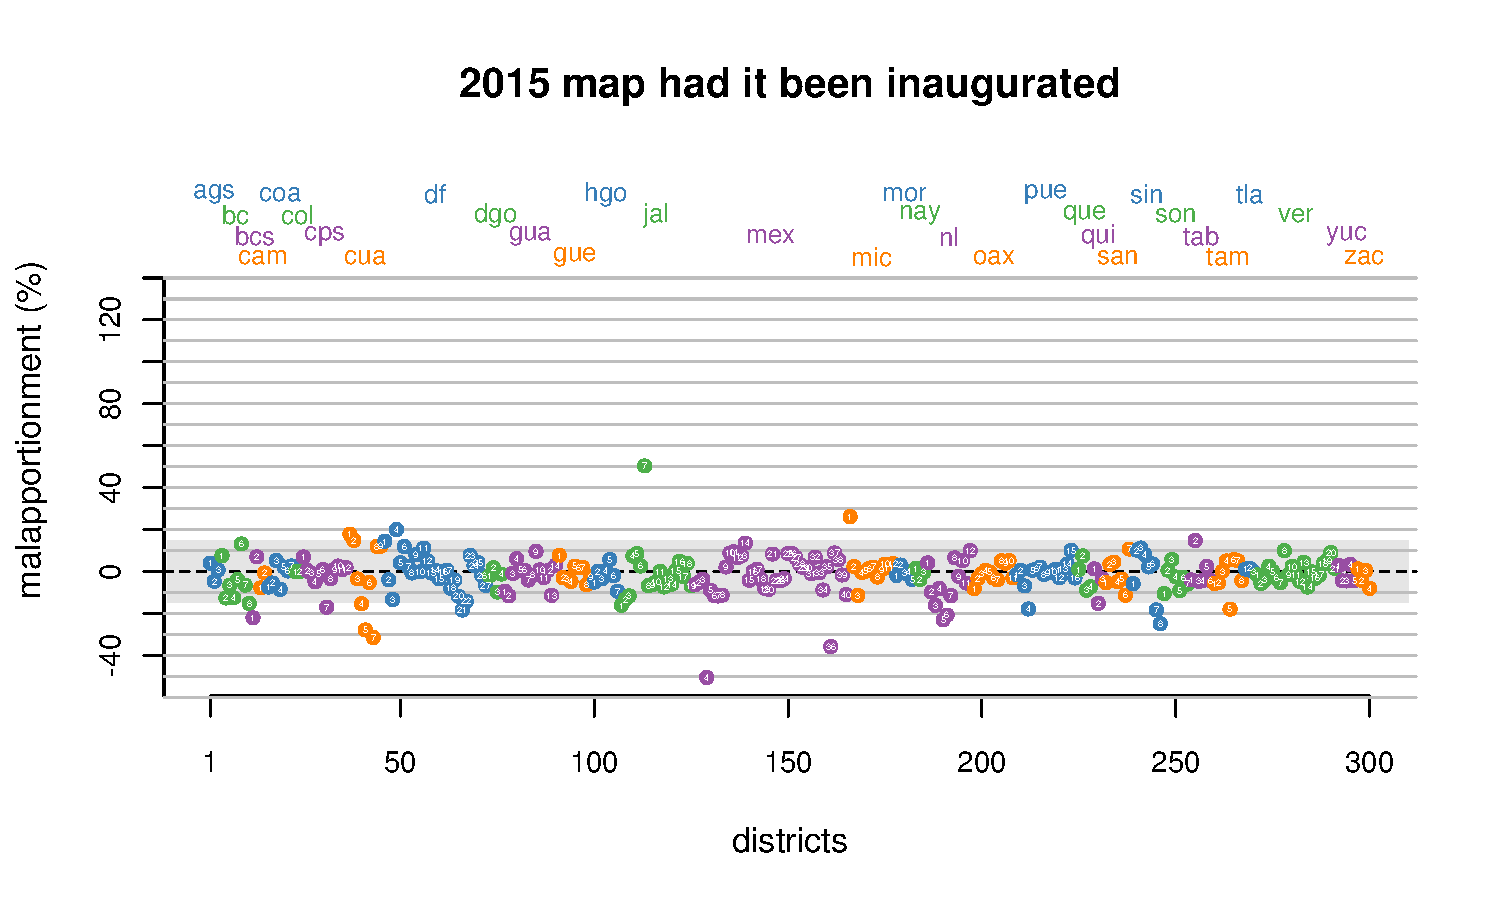
\includegraphics[width=12cm]{../graphs/malapp2015d3.pdf}
\end{center}

}
%%%%%%%%%%%%%%%%%%%%%%%%%%%%%%%%%%%%%%%%%%%%%%%%%%%%%%%%%%%%%%%%%%%%%%%%%%%%%%%%%%%%%%%%%%%% 

\frame {                      % SLIDE
    \frametitle{Malapportionment within states}

\begin{center}
   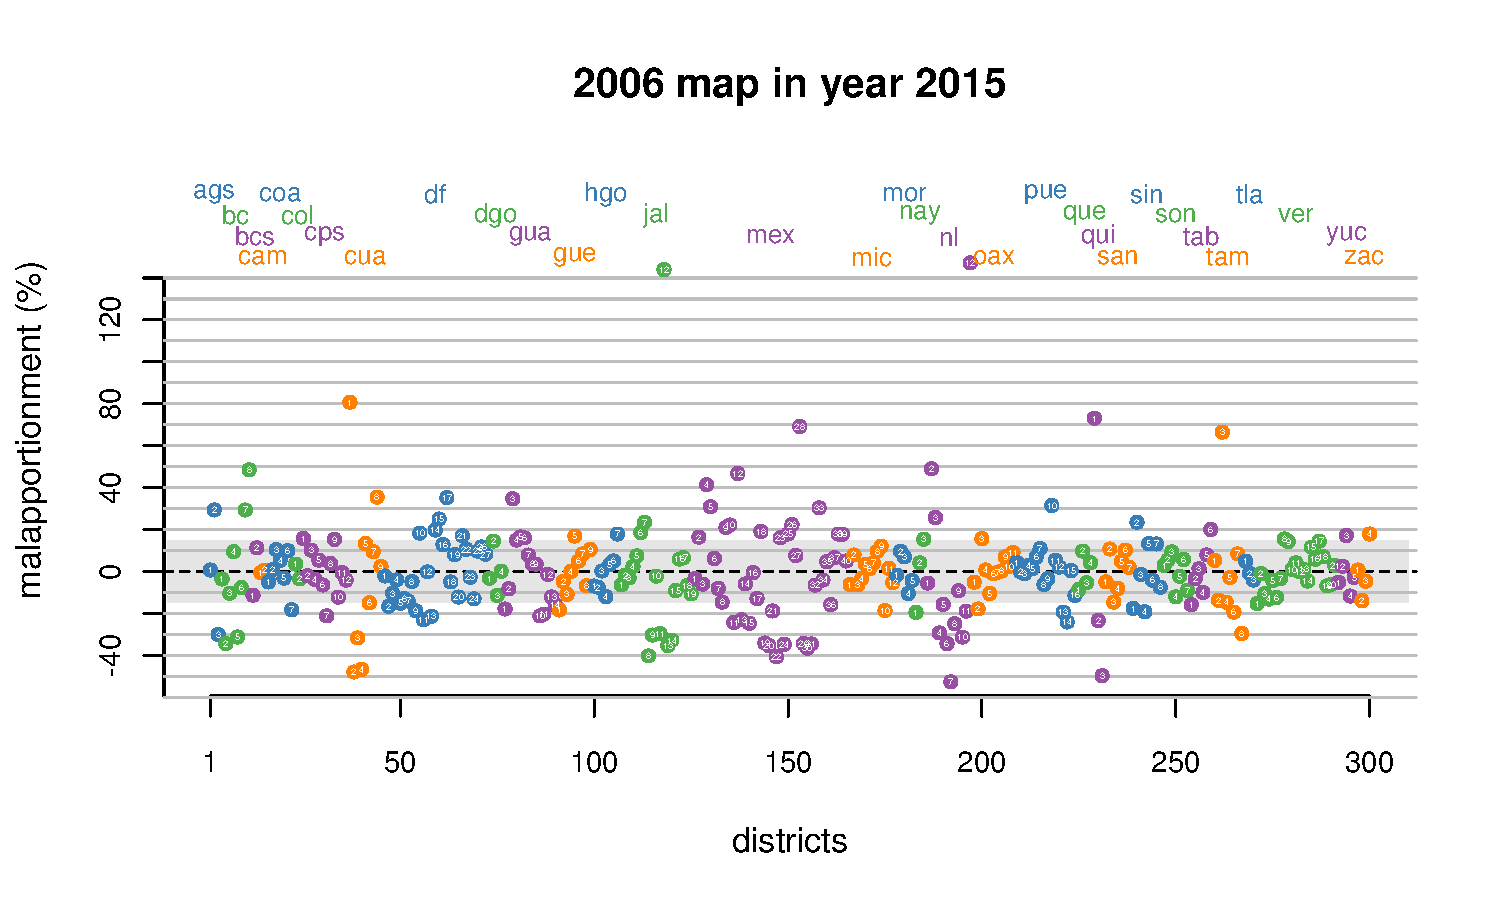
\includegraphics[width=12cm]{../graphs/malapp2015d0.pdf}
\end{center}

}
%%%%%%%%%%%%%%%%%%%%%%%%%%%%%%%%%%%%%%%%%%%%%%%%%%%%%%%%%%%%%%%%%%%%%%%%%%%%%%%%%%%%%%%%%%%% 

\frame {                      % SLIDE

    \frametitle{Two types of distortion}

Focus in the \alert{votes-to-seats} relation \\ (Rae 1967, Tufte 1973, Lijphart 1994, Taagepera\&Shugart 1989)

\bigskip

Two measures of interest:

\begin{enumerate}

\item \textbf{Party bias} $\lambda$: \\ helps beneficiary buy seats with fewer votes \\ (``packing'')

\item \textbf{Responsiveness} $\rho$: \\ seat bonus to large parties \\ (``microcosm strategy'')

\end{enumerate}

}

%%%%%%%%%%%%%%%%%%%%%%%%%%%%%%%%%%%%%%%%%%%%%%%%%%%%%%%%%%%%%%%%%%%%%%%%%%%%%%%%%%%%%%%%%%%% 

\frame {                      % SLIDE

    \frametitle{Two types of distortion}

\begin{center}
   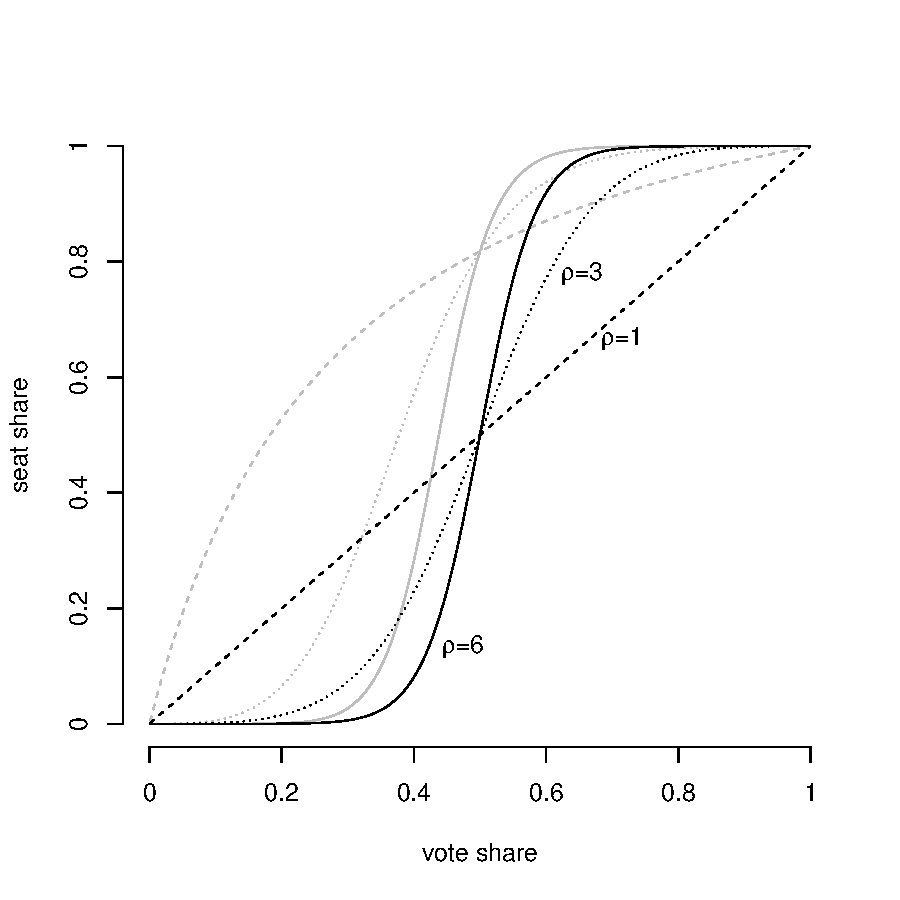
\includegraphics[width=8cm]{../graphs/rhoExample.pdf}
\end{center}

}
%%%%%%%%%%%%%%%%%%%%%%%%%%%%%%%%%%%%%%%%%%%%%%%%%%%%%%%%%%%%%%%%%%%%%%%%%%%%%%%%%%%%%%%%%%%% 

\frame {                      % SLIDE

    \frametitle{Formalization}

Cube Law:  \begin{equation*}  \frac{s}{1-s} = \left(\frac{v}{1-v}\right)^3 \end{equation*} 

\bigskip

Generalization (King\&Browning 1987):
\begin{equation*}
 \frac{s}{1-s} = e^\lambda *  \left(\frac{v}{1-v}\right)^\rho %\iff  \texttt{logit}(s) = \lambda + \rho *  \texttt{logit}(v)
\end{equation*}

\bigskip

Multiparty (King 1990, Calvo\&Micozzi 2005):
\begin{equation*}
 E(s_j) = \frac{e^{\lambda_j} * v_j^\rho}{\sum_{m=1}^{J} e^{\lambda_m} * v_m^\rho}
\end{equation*}


}

%%%%%%%%%%%%%%%%%%%%%%%%%%%%%%%%%%%%%%%%%%%%%%%%%%%%%%%%%%%%%%%%%%%%%%%%%%%%%%%%%%%%%%%%%%%% 

\frame {                      % SLIDE
    \frametitle{Data}

 \begin{columns}[c]

 \column{.8\textwidth}

\begin{center}
   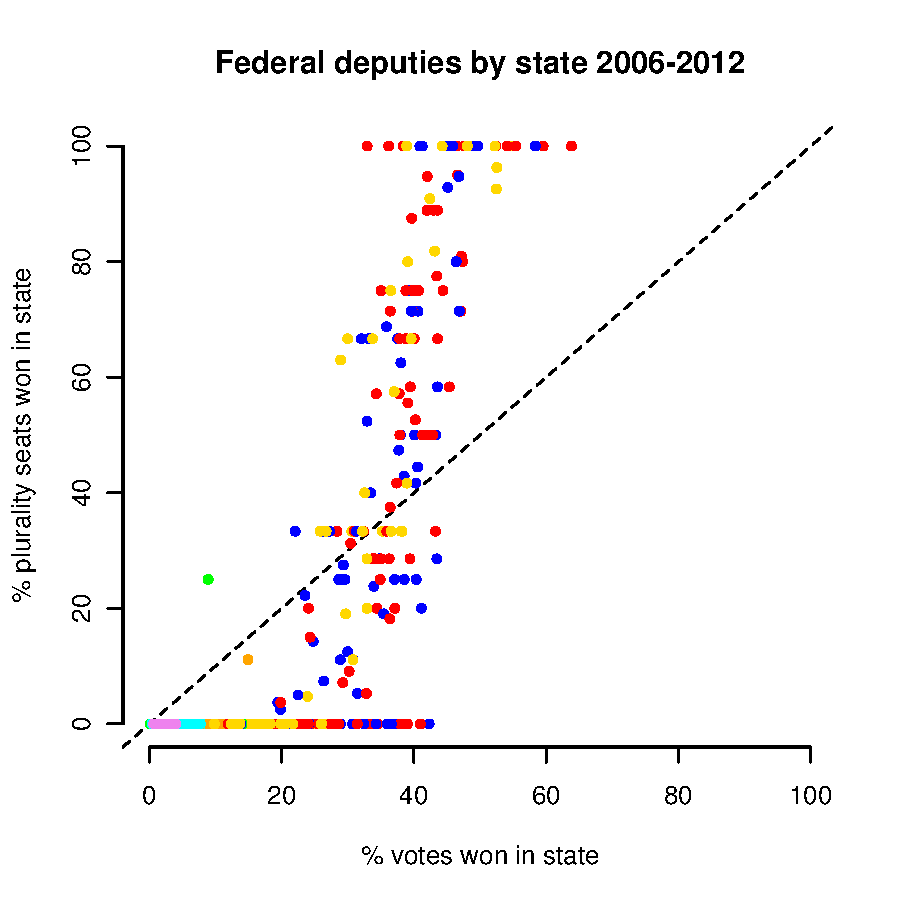
\includegraphics[width=6cm]{../graphs/resXedo20062012.pdf}
\end{center}

 \column{.2\textwidth}

{\color{blue} PAN} \\ {\color{red} PRI} \\ {\color{yellow} PRD} \\ {\color{green} Green}

\end{columns}

\begin{itemize}
\item State-level aggregates (average = 9.4 districts, but $\Delta^+N$) 
\item 2006--2012 districts constant
\item MCMC \footnotesize{($3 \times 10k$ iter., every $100^{th}$ for post.\ sample)}
\end{itemize}
}
%%%%%%%%%%%%%%%%%%%%%%%%%%%%%%%%%%%%%%%%%%%%%%%%%%%%%%%%%%%%%%%%%%%%%%%%%%%%%%%%%%%%%%%%%%%% 

\begin{frame}[fragile=singleslide]\frametitle{Bugs code}
\begin{tiny}
\begin{verbatim}
    for (i in 1:I){     # loop over state-years
        for (j in 1:J){ # loop over parties (dummy selects those who ran that year) 
            S[i,j] ~ dbin(pi[i,j], D[i])  # D is number SMD seats in obs. i's state
        }
        numerator[i,1] <- dummy[i,1] * exp( lambda[1] + rho * log(v[i,1]) )
        numerator[i,2] <- dummy[i,2] * exp(             rho * log(v[i,2]) )
        for (j in 3:J){
            numerator[i,j] <- dummy[i,j] * exp( lambda[j-1] ) * v[i,j]^rho
        }
        for (j in 1:J){ # loop over parties (dummy selects those who ran that year) 
            d1[i,j] <- dummy[i,1] * exp( lambda[1] ) * v[i,1]^rho 
            d2[i,j] <- dummy[i,2]                    * v[i,2]^rho 
            d3[i,j] <- dummy[i,3] * exp( lambda[2] ) * v[i,3]^rho 
            d4[i,j] <- dummy[i,4] * exp( lambda[3] ) * v[i,4]^rho 
            d5[i,j] <- dummy[i,5] * exp( lambda[4] ) * v[i,5]^rho 
            d6[i,j] <- dummy[i,6] * exp( lambda[5] ) * v[i,6]^rho 
            d7[i,j] <- dummy[i,7] * exp( lambda[6] ) * v[i,7]^rho 
            denominator[i,j] <- d1[i,j]+d2[i,j]+d3[i,j]+d4[i,j]+d5[i,j]+d6[i,j]+d7[i,j]
            pi[i,j] <- numerator[i,j] / denominator[i,j]
        }
    }
    ### priors
    for (p in 1:6){ # there are 7 party labels in the 3-election data, PRI is reference
        lambda[p] ~ dnorm( 0, tau.lambda )
    }
    tau.lambda <- pow(.25, -2)
    rho ~ dexp(.75) # this has positive range, median close to 1, mean 1.25, max 4.5
\end{verbatim}
\end{tiny}

\end{frame}

%%%%%%%%%%%%%%%%%%%%%%%%%%%%%%%%%%%%%%%%%%%%%%%%%%%%%%%%%%%%%%%%%%%%%%%%%%%%%%%%%%%%%%%%%%%% 

\frame {                      % SLIDE
    \frametitle{Presumption}

\begin{itemize}
\item PRI has strong bases of support in rural districts
\item rural districts under-populated
\item State-years above 45� line (2006--12): 
\end{itemize}

\begin{center}
\begin{tabular}{lr}
PRI & $^3/_5$ \\
PAN & $^2/_5$ \\
PRD & $^1/_4$ \\
\end{tabular}
\end{center}

\bigskip

\begin{block}{Johnston-like hypothesis:} 
Might malapportionment $\rightarrow$ bias in favor of PRI? \\ Against PAN? PRD?
\end{block}
}
%%%%%%%%%%%%%%%%%%%%%%%%%%%%%%%%%%%%%%%%%%%%%%%%%%%%%%%%%%%%%%%%%%%%%%%%%%%%%%%%%%%%%%%%%%%% 

\frame {                      % SLIDE
    \frametitle{Results: party bias}
\begin{center}
\begin{tabular}{cc}
   2006 map & 2015 map \\
   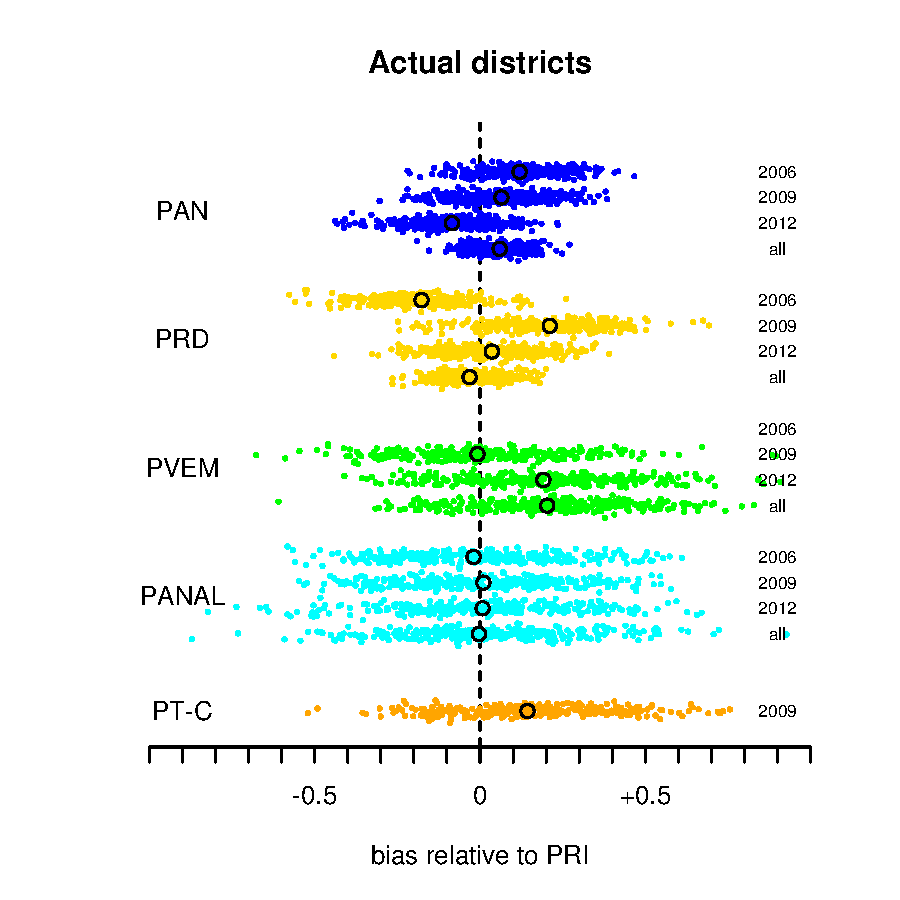
\includegraphics[width=5cm]{../graphs/bias200612s0.pdf} &
   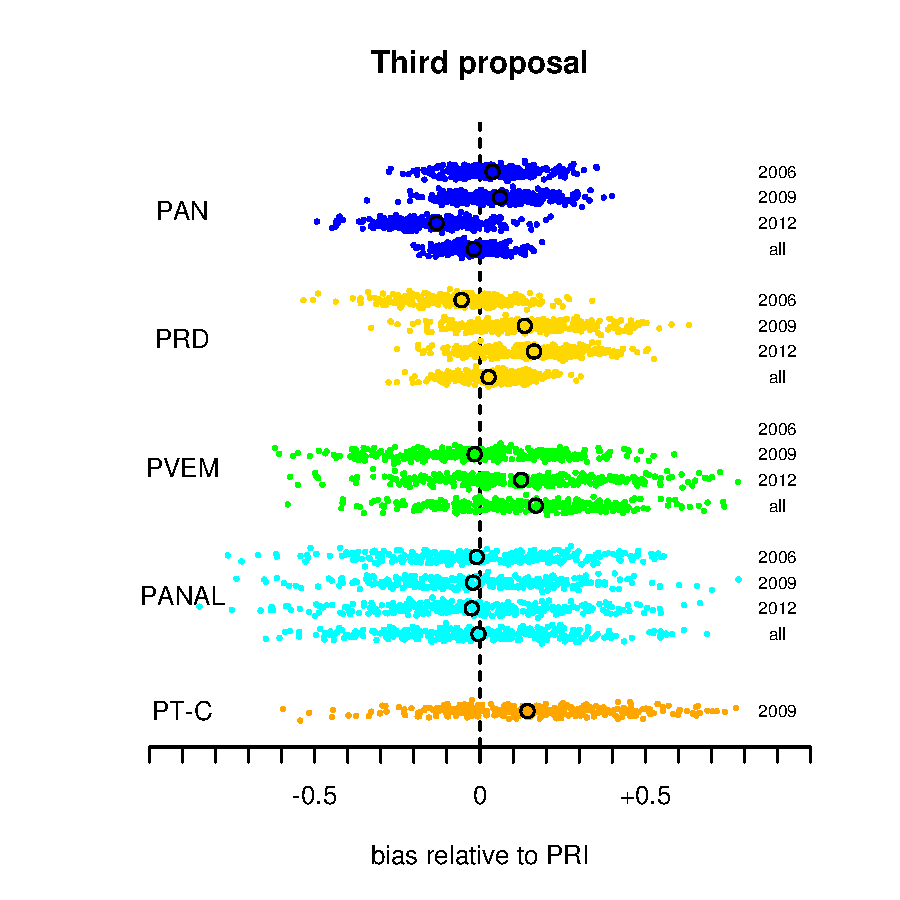
\includegraphics[width=5cm]{../graphs/bias200612s3.pdf}
\end{tabular}
\end{center}
}
%%%%%%%%%%%%%%%%%%%%%%%%%%%%%%%%%%%%%%%%%%%%%%%%%%%%%%%%%%%%%%%%%%%%%%%%%%%%%%%%%%%%%%%%%%%% 

\frame {                      % SLIDE
    \frametitle{Results: responsiveness}
\begin{center}
   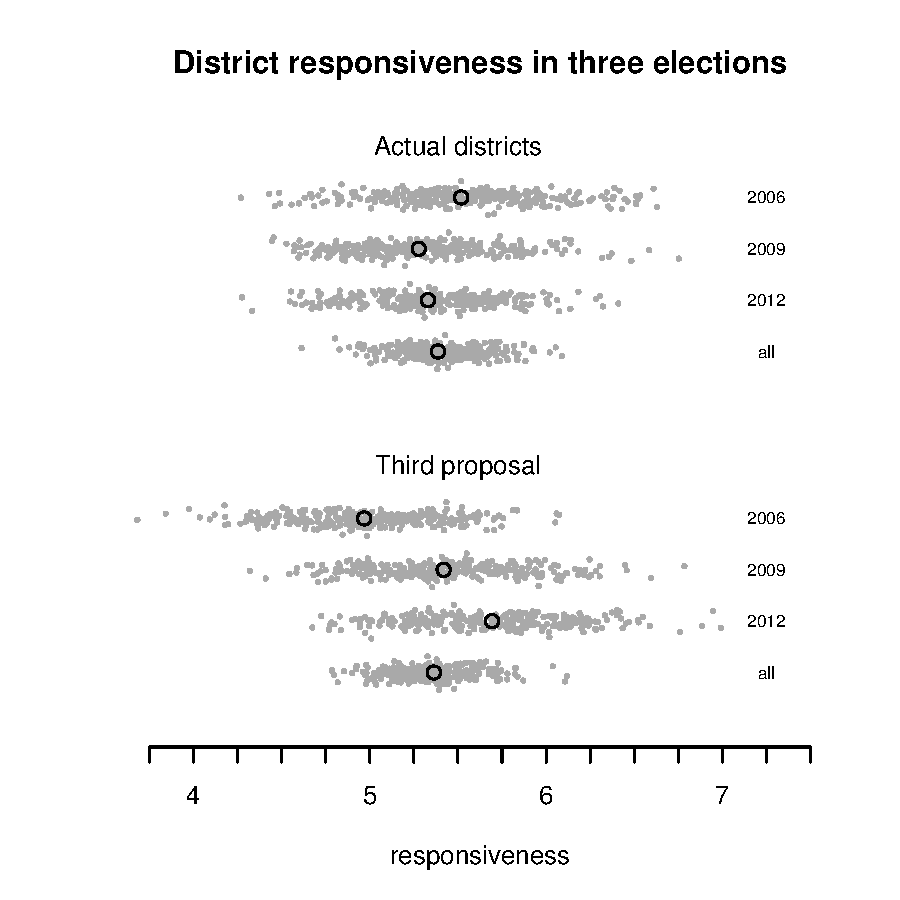
\includegraphics[width=6cm]{../graphs/resp200612s0s3.pdf}
\end{center}
}
%%%%%%%%%%%%%%%%%%%%%%%%%%%%%%%%%%%%%%%%%%%%%%%%%%%%%%%%%%%%%%%%%%%%%%%%%%%%%%%%%%%%%%%%%%%%%%%%

\frame {                      % SLIDE

    \frametitle{Findings, next steps}

Preliminary analysis reveals that:

\begin{enumerate}

\item Substantial malapportionent

\item No evidence of systematic party bias

\item Huge large-party bonus (PRI is small in few states)

\item Are effects of malapp.\ eclipsed by inter-election volatility?

\item Study residuals from estimation: relation to \\ malapp.? turnout diff.? geography of support?

\item Larger project     \hyperlink{fr:MxMapProj}{\beamergotobutton{Link}}


\end{enumerate}

\pause

\bigskip

\center{\textbf{\Large{Thank you!}}}

}
\end{document}

%%%%%%%%%%%%%%%%%%%%%%%%%%%%%%%%%%%%%%%%%%%%%%%%%%%%%%%%%%%%%%%%%%%%%%%%%%%%%%%%%%%%%%%%%%%%
\frame {                      % SLIDE
    \frametitle{Tit}
}
